\section{Sprint 4}
\subsection{Introduction}
This sprint focused on developing advanced AI analytics and intelligent features for MindCareAI.
It included AI analytics warehouse, AI engine services, crisis monitoring system, AI-powered custom feeds, toxic content detection, enhanced chatbot with RAG system, and enhanced notifications.
Advanced data processing, machine learning algorithms, and real-time monitoring capabilities were implemented.
These features aim to provide intelligent mental health support through advanced analytics and AI-driven insights.

\subsection{Sprint Backlog}
\begin{longtable}{|p{4.2cm}|p{7.2cm}|p{2.2cm}|}
\hline
\textbf{User Story} & \textbf{Task} & \textbf{Priorities} \\
\hline
\endfirsthead
\hline
\textbf{User Story} & \textbf{Task} & \textbf{Priorities} \\
\hline
\endhead
\hline
\multicolumn{3}{|r|}{\textit{Continued on next page}} \\
\hline
\endfoot
\hline
\endlastfoot
As a therapist, I want comprehensive data collection & Implement AI Analytics Warehouse with PostgreSQL, Redis Streams and real-time data aggregation from 7+ sources (mood, journal, therapy, messaging, medical) & High \\
\hline
As a therapist, I want secure data processing & Create enterprise ETL pipeline with AES encryption, audit trails, incremental/full backups, HIPAA compliance, and automated integrity validation & High \\
\hline
As a therapist, I want real-time analytics & Add real-time analytics with Redis Streams, WebSocket events, anomaly detection algorithms, and live dashboard updates (sub-second processing) & Medium \\
\hline
As a therapist, I want customizable reports & Build dynamic reporting system with PDF generation, customizable timeframes, statistical analysis, and exportable CSV/JSON formats & Medium \\
\hline
As a therapist, I want AI conversation summaries & Implement conversation summary service using Ollama Mistral 7B LLM, therapeutic insight extraction, action item identification, and sentiment analysis & High \\
\hline
As a therapist, I want medication analysis & Add medication adherence analysis with statistical models, side effect correlation, dosage effectiveness tracking, and predictive adherence scoring & High \\
\hline
As a therapist, I want predictive analytics & Create ML predictive services using time-series analysis, ARIMA models, mood decline prediction, therapy outcome forecasting, and risk assessment algorithms & High \\
\hline
As a therapist, I want social interaction insights & Implement social interaction analysis using NetworkX graph algorithms, relationship mapping, communication pattern detection, and social network analysis & Medium \\
\hline
As a therapist, I want crisis detection & Build real-time crisis monitoring with SpaCy NLP, keyword pattern matching, weighted confidence scoring, and multi-level alert system & High \\
\hline
As a therapist, I want crisis management & Add automatic crisis level determination with intervention workflows, escalation paths, therapist notifications, and emergency contact systems & High \\
\hline
As a therapist, I want emergency alerts & Implement emergency notification system with WebSocket real-time alerts, SMS integration, email escalation, and priority-based routing & High \\
\hline
As a therapist, I want crisis tracking & Create historical crisis tracking with pattern identification, trend analysis, risk factor correlation, and predictive crisis modeling & Medium \\
\hline
As a patient, I want personalized content & Implement AI-powered custom feeds with collaborative filtering, content-based recommendations, mood-state matching, and Thompson sampling for diversity & Medium \\
\hline
As a patient, I want mood-based suggestions & Add mood-based content suggestion using emotion detection models, sentiment analysis, therapeutic content matching, and personalized tip generation & Medium \\
\hline
As a patient, I want content variety & Create content diversity mechanisms with topic distribution analysis, echo chamber prevention algorithms, and balanced content exposure strategies & Low \\
\hline
As a therapist, I want toxic content detection & Implement pattern recognition using Google Perspective API, custom NLP models, toxicity scoring, automatic content flagging, and multi-language support & High \\
\hline
As a therapist, I want automated moderation & Add multi-level content moderation with confidence scoring, automated blocking, manual review queues, and escalation workflows & High \\
\hline
As a therapist, I want moderation dashboard & Build comprehensive moderation dashboard with toxicity heatmaps, review queues, action logs, and performance analytics & Medium \\
\hline
As a patient, I want enhanced chatbot & Implement enhanced chatbot with RAG system using pgvector embeddings, HNSW indexing, Ollama LLM integration, and contextual therapy recommendations & High \\
\hline
As a therapist, I want crisis detection in chat & Add real-time crisis detection in chatbot with weighted confidence scoring, immediate intervention triggers, and automated therapist alerts & High \\
\hline
As a patient, I want personalized responses & Implement response humanization with personality adaptation, therapeutic tone adjustment, personalized examples, and context-aware communication styles & Medium \\
\hline
As a patient, I want enhanced notifications & Build enhanced notification system with WebSocket real-time delivery, scheduled reminders, preference management, and multi-channel distribution & Medium \\
\caption{Sprint 4 Backlog -- AI Analytics \& Advanced Features}
\end{longtable}

\subsubsection{Functional Analysis}
\begin{figure}[H]
    \centering
    \includegraphics[width=0.9\textwidth]{images/chapter 5/srpint4_use_cases.drawio.png}
    \caption{Sprint 4 - Use Case Diagram for Sprint 4}
    \label{fig:use_case_sprint4}
\end{figure}

\begin{longtable}{|p{3cm}|p{12cm}|}
\hline
\textbf{Field} & \textbf{Details} \\
\hline
Title & AI Analytics Warehouse \\
\hline
Actor & Therapist, Patient \\
\hline
Description & System collects comprehensive data from diverse sources and processes it through secure ETL pipelines with real-time analytics capabilities and customizable reporting \\
\hline
Condition & System must have access to data sources and processing infrastructure \\
\hline
Output & Integrated data warehouse, real-time analytics, customizable reports, data quality validation \\
\hline
Scenario & 1. Data collection from mood tracking, journaling, messaging, therapy sessions \newline 2. ETL pipeline processes data with batch and incremental processing \newline 3. Real-time analytics processing using Redis Streams \newline 4. Quality reporting with automated validation \newline 5. Customizable reporting generation for therapists \newline 6. Data warehouse audit and backup protocols \\
\hline
Error handling & Data source connection failures, ETL processing errors, real-time stream interruptions, report generation failures, backup and security issues \\
\hline
\caption{AI Analytics Warehouse Use Case}
\end{longtable}

\begin{longtable}{|p{3cm}|p{12cm}|}
\hline
\textbf{Field} & \textbf{Details} \\
\hline
Title & AI Engine Services \\
\hline
Actor & Therapist, Patient, System \\
\hline
Description & AI-powered services including conversation summaries, medication analysis, predictive analytics, and social interaction analysis using advanced machine learning algorithms \\
\hline
Condition & System must have access to AI models and patient data \\
\hline
Output & Therapeutic conversation summaries, medication adherence insights, mental health trend predictions, social interaction analysis \\
\hline
Scenario & 1. Conversation summaries generated using Ollama and Mistral LLM \newline 2. Medication analysis tracks adherence using statistical models \newline 3. Predictive services analyze mental health trends \newline 4. Social interaction analysis using Pearson Correlation and graph algorithms \newline 5. Therapy analysis provides treatment recommendations \newline 6. Multi-modal data integration for holistic patient profiles \\
\hline
Error handling & AI model processing failures, data integration errors, statistical analysis issues, prediction accuracy problems, social graph computation errors \\
\hline
\caption{AI Engine Services Use Case}
\end{longtable}

\begin{longtable}{|p{3cm}|p{12cm}|}
\hline
\textbf{Field} & \textbf{Details} \\
\hline
Title & Crisis Monitoring System \\
\hline
Actor & Therapist, Patient \\
\hline
Description & Real-time crisis detection, automatic risk assessment, emergency notifications, and intervention workflow management with historical tracking capabilities \\
\hline
Condition & System must have access to patient communications and healthcare provider network \\
\hline
Output & Real-time crisis alerts, risk level assessments, emergency notifications, intervention workflows, historical crisis patterns \\
\hline
Scenario & 1. Monitoring communications for crisis indicators using NLP \newline 2. Automatic crisis level determination using BERT-based classification \newline 3. Immediate response triggers for high-risk situations \newline 4. Emergency notification system alerts therapists \newline 5. Intervention workflow management with role-based assignments \newline 6. Historical crisis tracking for pattern identification \\
\hline
Error handling & NLP processing failures, crisis classification errors, notification delivery failures, workflow assignment issues, historical data analysis problems \\
\hline
\caption{Crisis Monitoring System Use Case}
\end{longtable}

\begin{longtable}{|p{3cm}|p{12cm}|}
\hline
\textbf{Field} & \textbf{Details} \\
\hline
Title & AI-Powered Custom Feeds \\
\hline
Actor & Patient, Therapist \\
\hline
Description & Personalized content recommendations based on mood, topics, and user behavior using advanced machine learning algorithms and feedback loops \\
\hline
Condition & Patient must be authenticated and have interaction history \\
\hline
Output & Personalized content recommendations, topic-based feeds, mood-aligned suggestions, engagement-driven content refresh \\
\hline
Scenario & 1. Analysis of user behavior and preferences \newline 2. Content-based filtering using TF-IDF vectorization \newline 3. Topic-based customization using SpaCy NLP \newline 4. Mood-based suggestions using RoBERTa emotion detection \newline 5. AI feedback loop for recommendation improvement \newline 6. Content diversity mechanisms prevent echo chambers \\
\hline
Error handling & Recommendation algorithm failures, topic extraction errors, mood detection issues, feedback loop problems, content diversity imbalances \\
\hline
\caption{AI-Powered Custom Feeds Use Case}
\end{longtable}

\begin{longtable}{|p{3cm}|p{12cm}|}
\hline
\textbf{Field} & \textbf{Details} \\
\hline
Title & Toxic Content Detection \\
\hline
Actor & Therapist \\
\hline
Description & Comprehensive toxic content detection using Google Perspective API, automated moderation with confidence scoring, and manual review capabilities \\
\hline
Condition & System must have access to Google Perspective API and content streams \\
\hline
Output & Automated content filtering, toxicity confidence scores, moderation dashboard alerts, educational content redirects \\
\hline
Scenario & 1. Scanning content using Google Perspective API \newline 2. Pattern recognition for harmful language detection \newline 3. Multi-level content moderation with confidence scoring \newline 4. Automatic filtering of harmful content \newline 5. User reporting system with AI verification \newline 6. Moderation dashboard for therapist review \\
\hline
Error handling & API connection failures, false positive detection, confidence scoring errors, moderation workflow issues, dashboard display problems \\
\hline
\caption{Toxic Content Detection Use Case}
\end{longtable}

\begin{longtable}{|p{3cm}|p{12cm}|}
\hline
\textbf{Field} & \textbf{Details} \\
\hline
Title & Enhanced Chatbot with RAG System \\
\hline
Actor & Patient \\
\hline
Description & Advanced chatbot capabilities with Retrieval-Augmented Generation using pgvector, HNSW indexing, crisis detection, and personalized therapeutic responses \\
\hline
Condition & Patient must be authenticated and system must have access to therapy knowledge base \\
\hline
Output & Therapy approach recommendations, crisis detection alerts, personalized responses, secure conversation history \\
\hline
Scenario & 1. Patient initiates conversation with enhanced chatbot \newline 2. RAG with pgvector and HNSW indexing for therapy recommendations \newline 3. Conversation context management with session state \newline 4. Crisis detection with weighted confidence scoring \newline 5. Response humanization and personalization \newline 6. Multi-session context awareness with secure history \\
\hline
Error handling & Vector database connection issues, RAG retrieval failures, crisis detection false positives, personalization errors, context management problems \\
\hline
\caption{Enhanced Chatbot with RAG System Use Case}
\end{longtable}

\begin{longtable}{|p{3cm}|p{12cm}|}
\hline
\textbf{Field} & \textbf{Details} \\
\hline
Title & Enhanced Notifications \\
\hline
Actor & Patient, Therapist \\
\hline
Description & Comprehensive notification capabilities including real-time WebSocket alerts, scheduled reminders, crisis notifications, and platform-wide announcements \\
\hline
Condition & Users must be authenticated and have notification permissions enabled \\
\hline
Output & Real-time WebSocket notifications, scheduled reminders, crisis alerts, medication compliance notifications, system announcements \\
\hline
Scenario & 1. Monitoring events requiring notifications \newline 2. Direct message and group communication alerts via WebSocket \newline 3. Personalized tips and mental health reminders \newline 4. Crisis alert system for therapists \newline 5. Medication and therapy compliance reminders \newline 6. Platform-wide announcement capabilities \\
\hline
Error handling & WebSocket connection failures, scheduling system errors, notification delivery issues, compliance tracking problems, announcement broadcast failures \\
\hline
\caption{Enhanced Notifications Use Case}
\end{longtable}

\newpage

\subsection{Database Design}

This subsection presents the database schema used in the system. The design ensures data integrity, scalability, and normalization for advanced AI analytics and monitoring features.
 
\vfill
\begin{figure}[H]
    \centering
    \includegraphics[width=1\textheight, height=0.55\textwidth, angle=90]{images/chapter 5/sprint4_database_erd.png}
    \caption{Database Design Diagram}
    \label{fig:database-design-sprint4}
\end{figure}

\vfill
\newpage

\subsection{Software Design}

This section provides a structural and behavioral view of the software system using UML diagrams.

\paragraph{Class Diagram}

The class diagram outlines the static structure of the system, detailing the classes, attributes, methods, and relationships for Sprint 4 features.

\begin{figure}[H]
    \centering
    \includegraphics[width=1\textwidth]{images/chapter 5/Sprint4_Class_Diagramv2.png}
    \caption{Class Diagram of the System}
    \label{fig:class-diagram-sprint4}
\end{figure}

\paragraph{Sequence Diagrams}

The following sequence diagrams illustrate the dynamic behavior of each major system component in Sprint 4, focusing on object interactions over time for each Django application.

\begin{figure}[H]
    \centering
    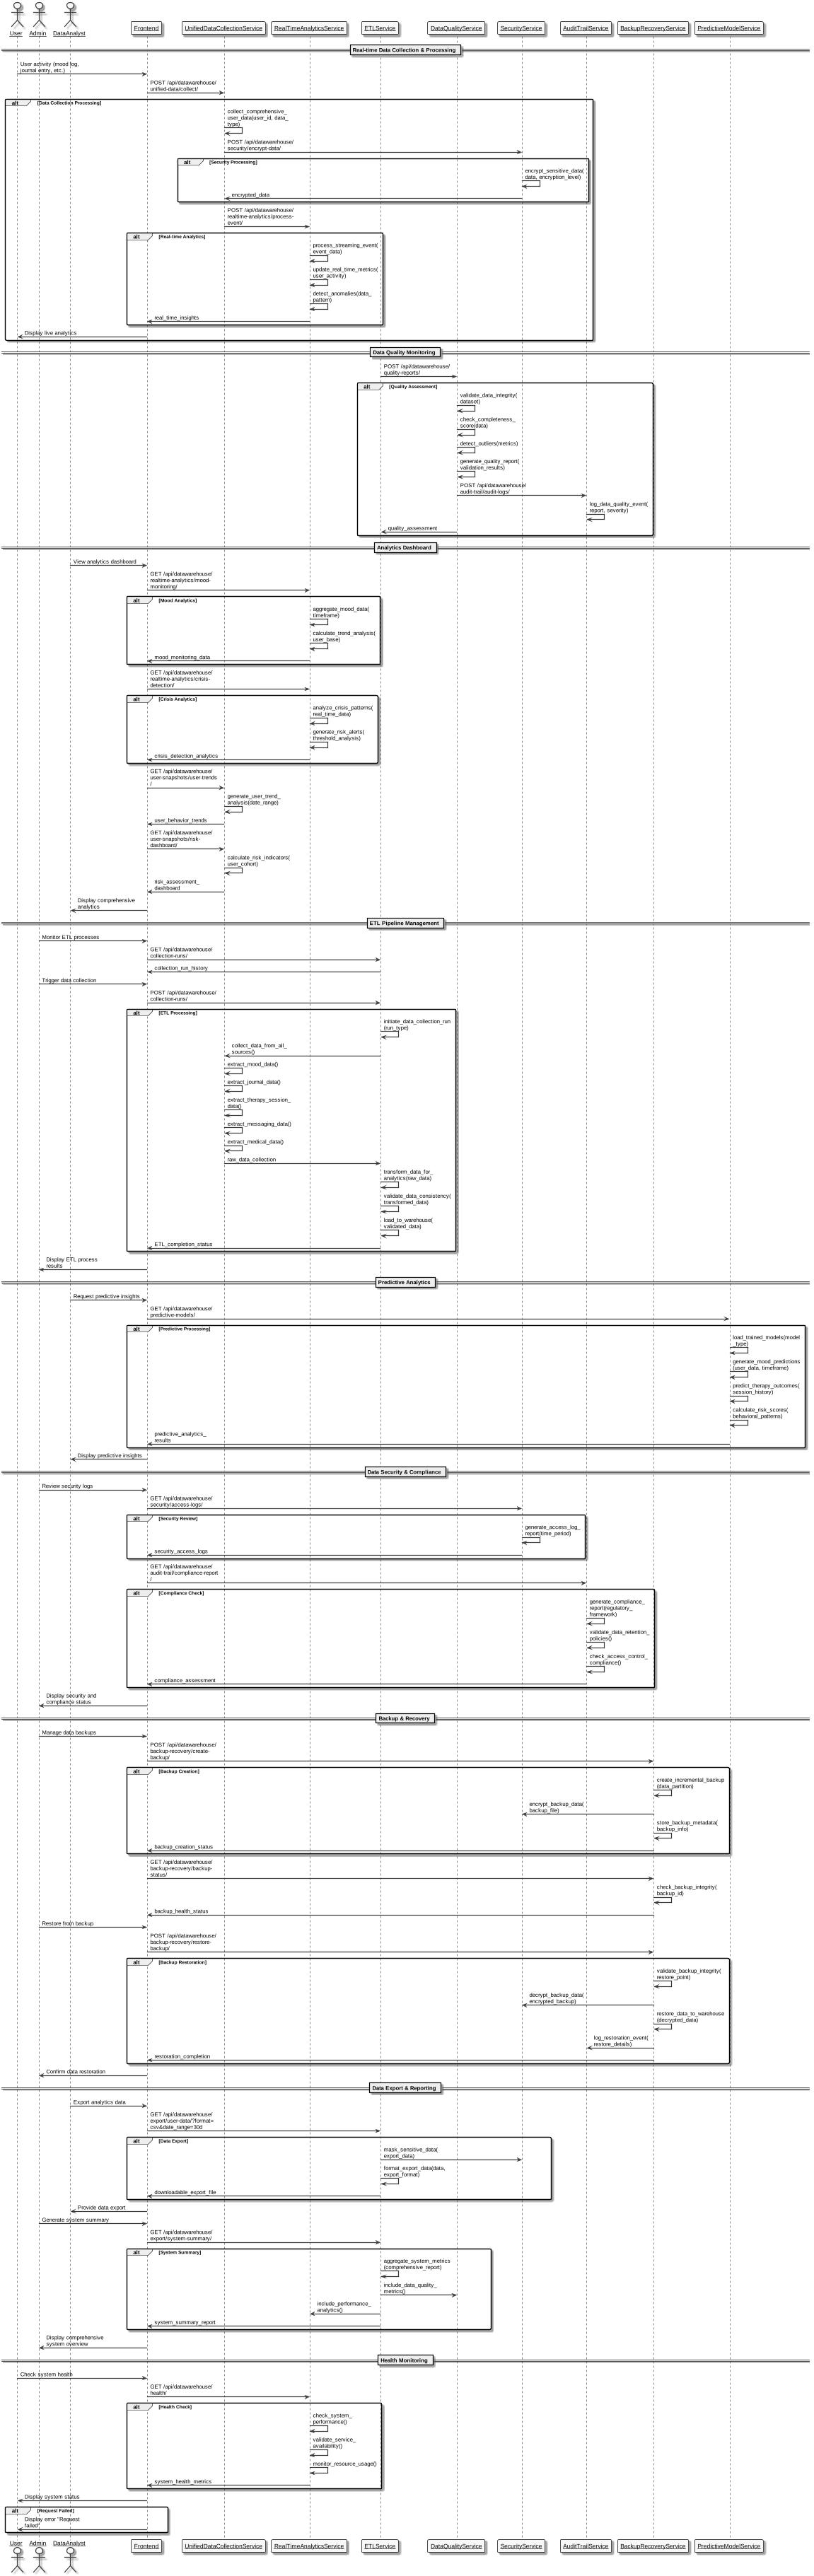
\includegraphics[width=0.9\textwidth]{images/chapter 5/sprint 4/Datawarehouse_Sequence_Diagram.png}
    \caption{Data Warehouse - Data Collection \& Processing}
    \label{fig:Datawarehouse-sequence-diagram}
\end{figure}

\begin{figure}[H]
    \centering
    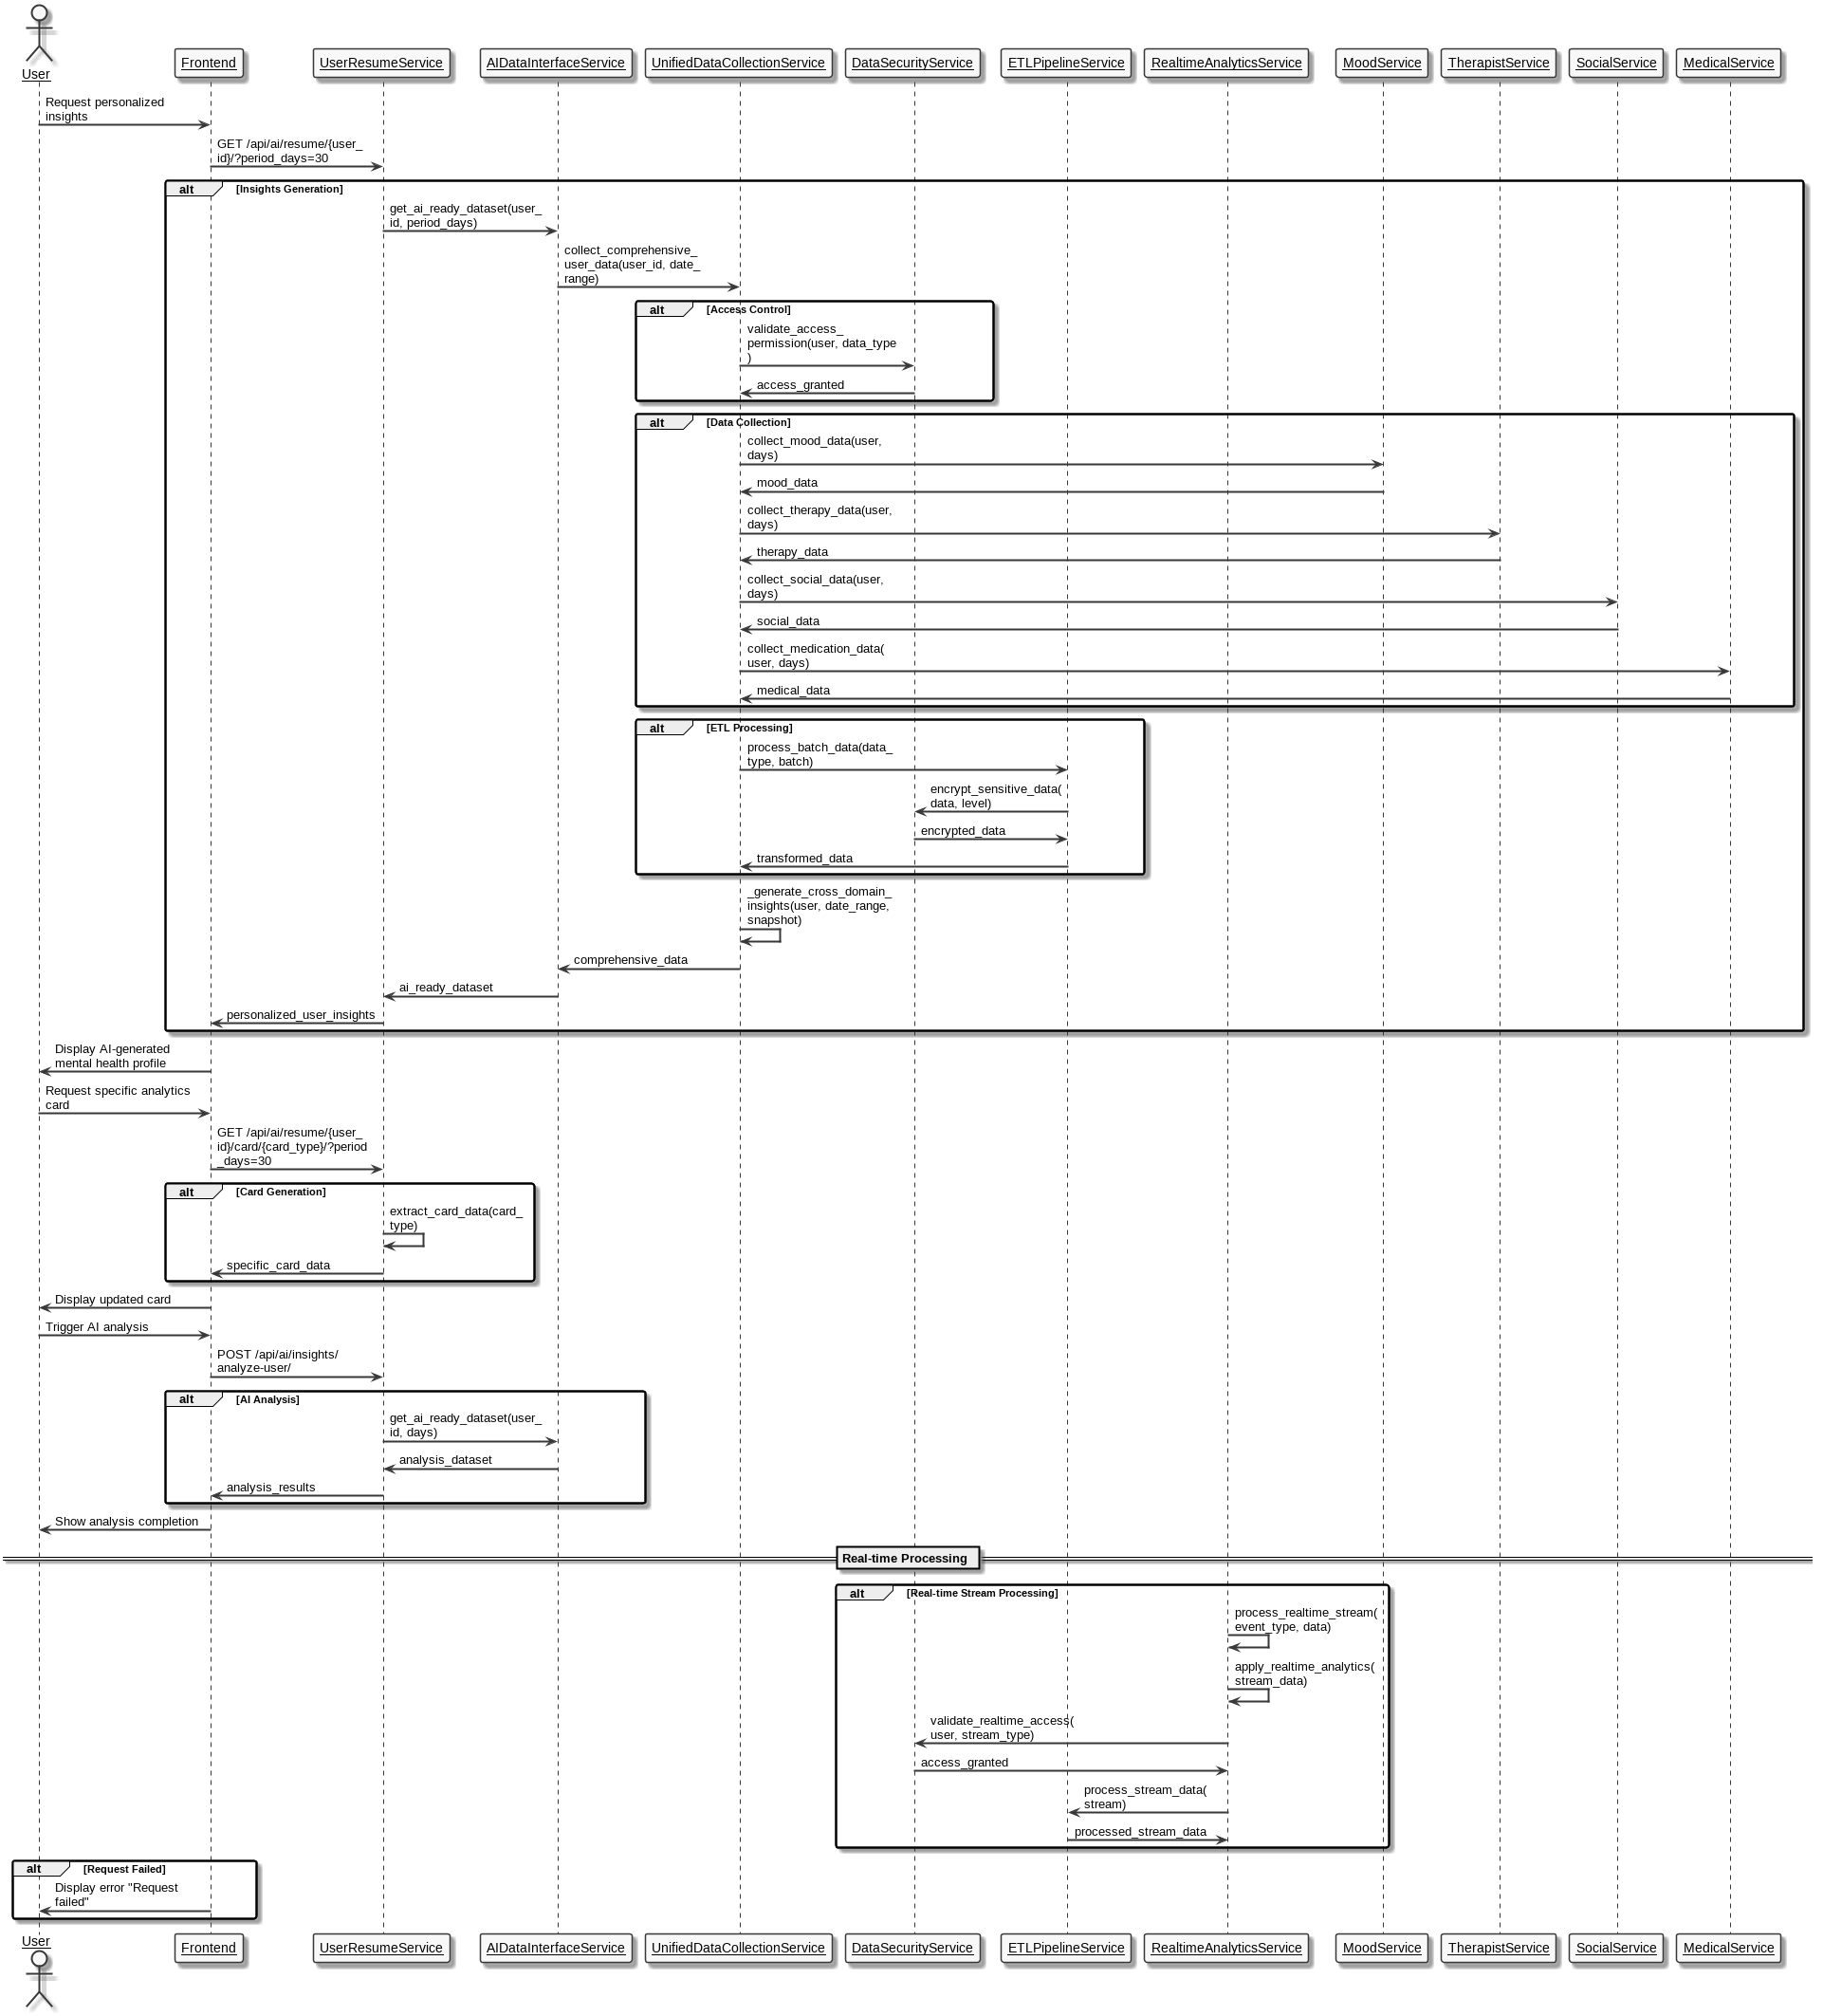
\includegraphics[width=0.8\textwidth]{images/chapter 5/sprint 4/Analytics_Sequence_Diagram.png}
    \caption{Data analytics}
    \label{fig:analytics-sequence-diagram}
\end{figure}

\begin{figure}[H]
    \centering
    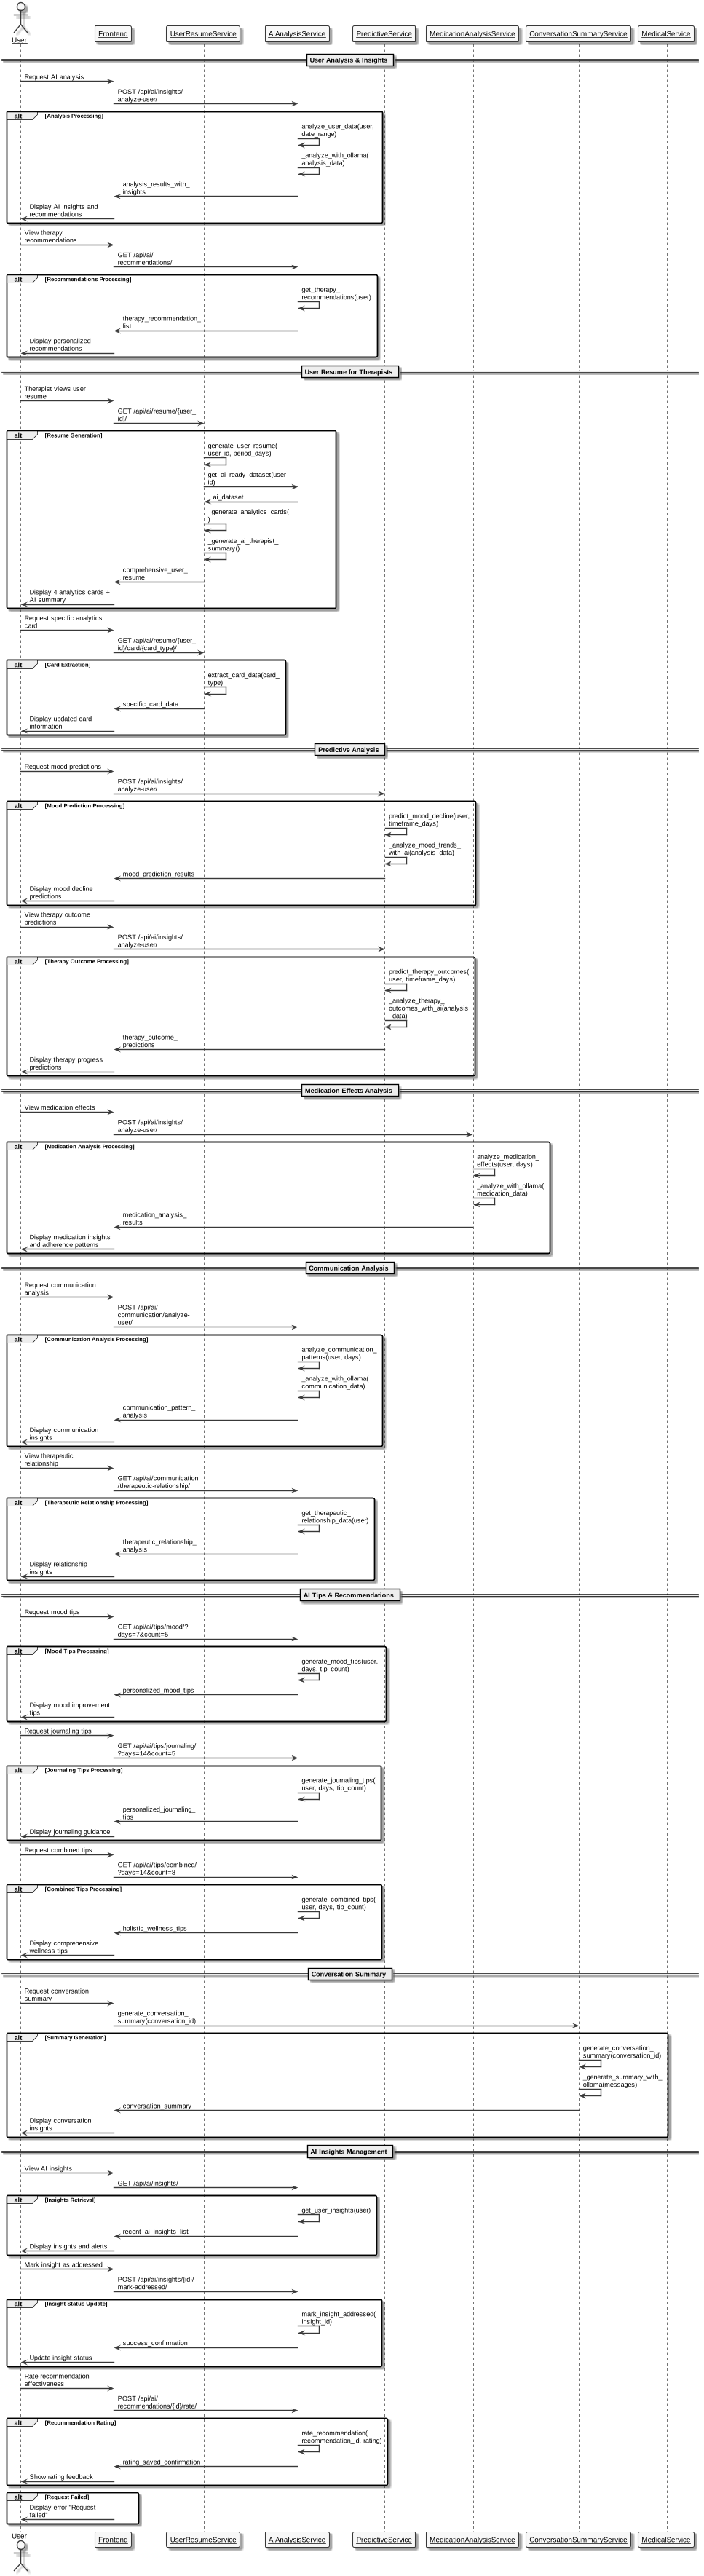
\includegraphics[width=0.65\textwidth]{images/chapter 5/sprint 4/AI_Engine_Sequence_Diagram.png}
    \caption{AI Engine Services - Analysis \& Predictions}
    \label{fig:ai-engine-sequence-diagram}
\end{figure}

\begin{figure}[H]
    \centering
    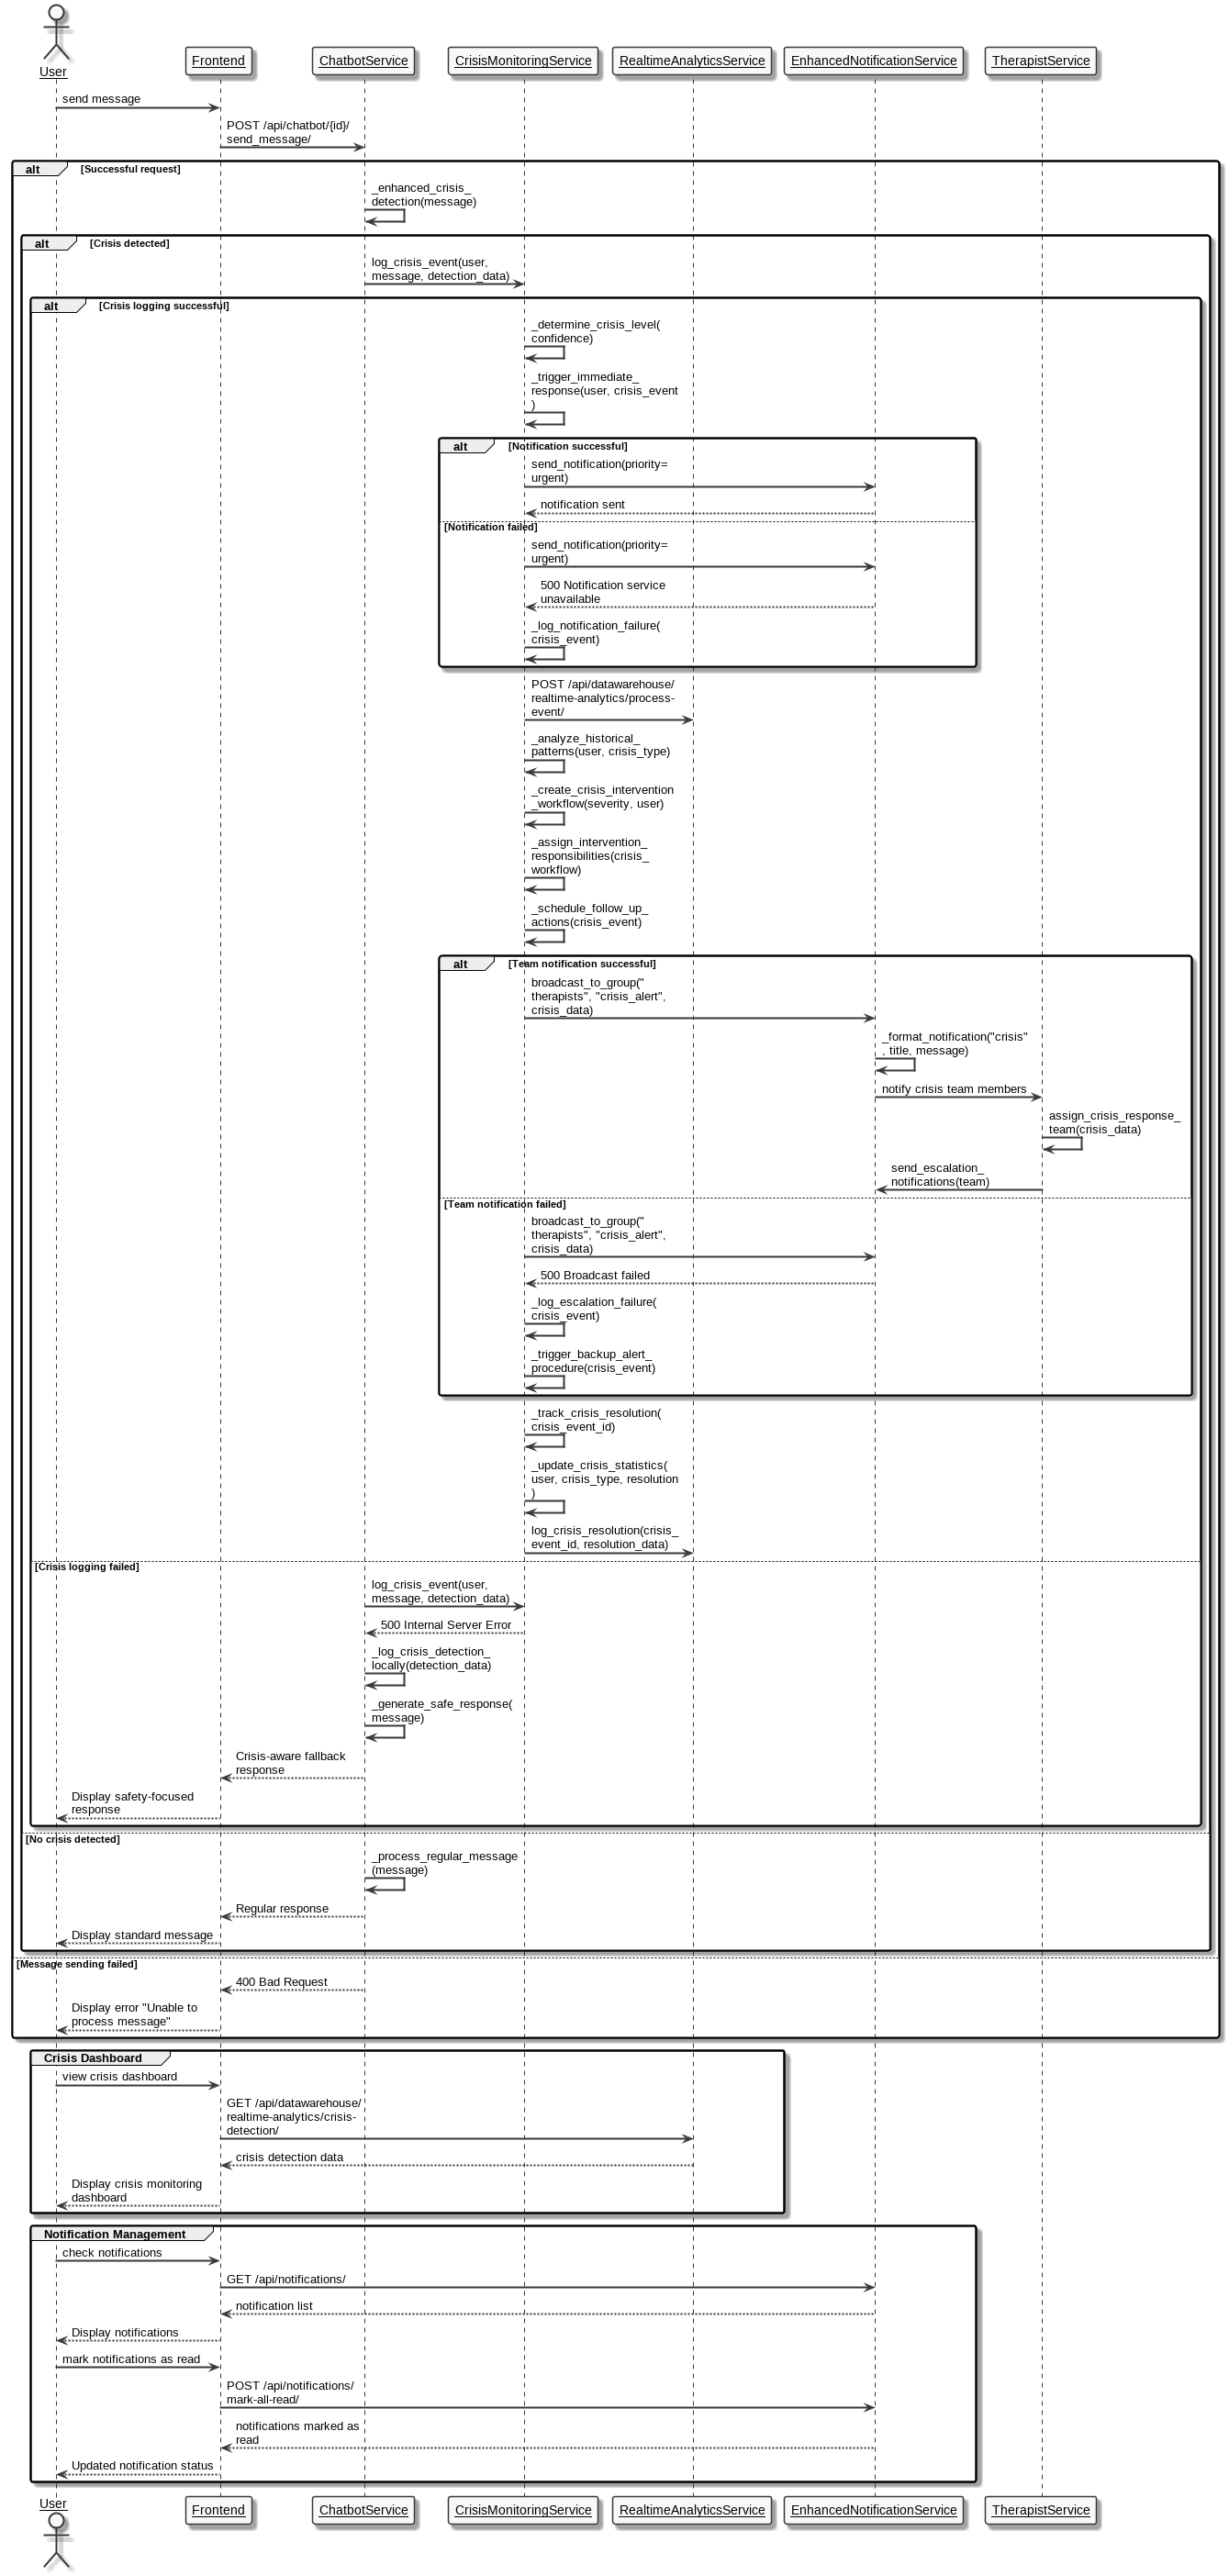
\includegraphics[width=0.75\textwidth]{images/chapter 5/sprint 4/Crisis_Monitoring_Sequence_Diagram.png}
    \caption{Crisis Monitoring System - Detection \& Response}
    \label{fig:crisis-monitoring-sequence-diagram}
\end{figure}

\begin{figure}[H]
    \centering
    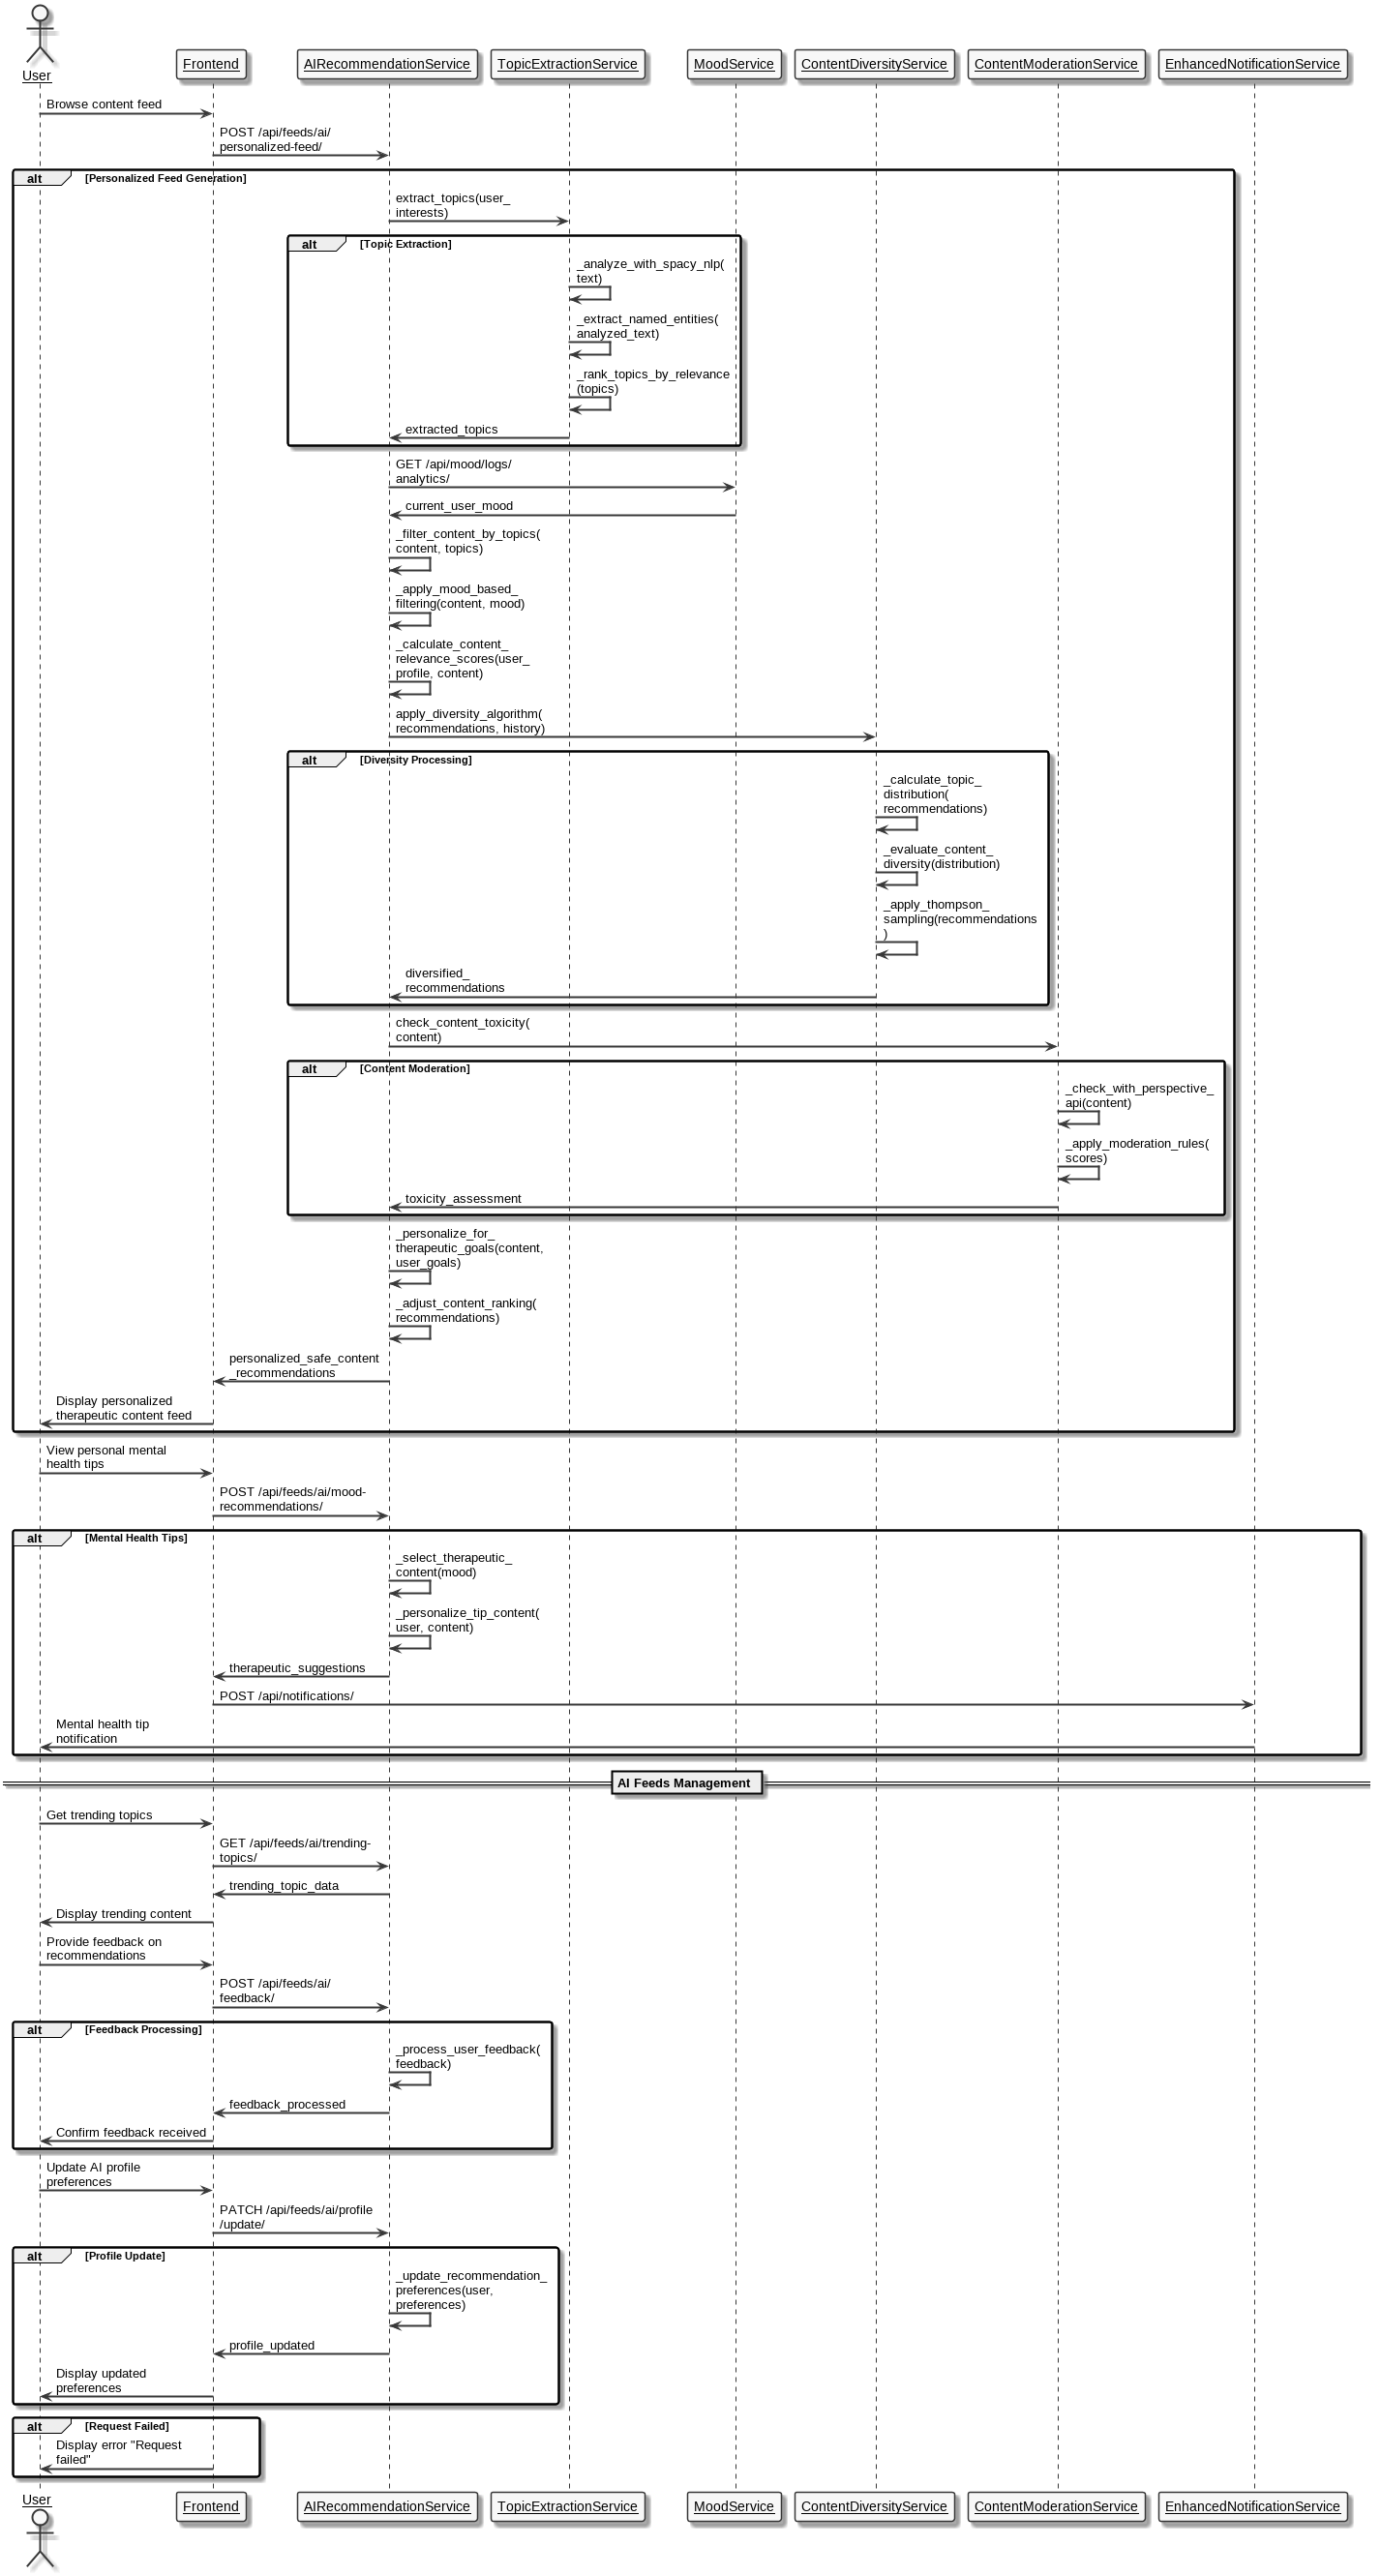
\includegraphics[width=0.75\textwidth]{images/chapter 5/sprint 4/Feeds_Sequence_Diagram.png}
    \caption{AI-Powered Custom Feeds - Content Recommendations}
    \label{fig:feeds-sequence-diagram}
\end{figure}

\begin{figure}[H]
    \centering
    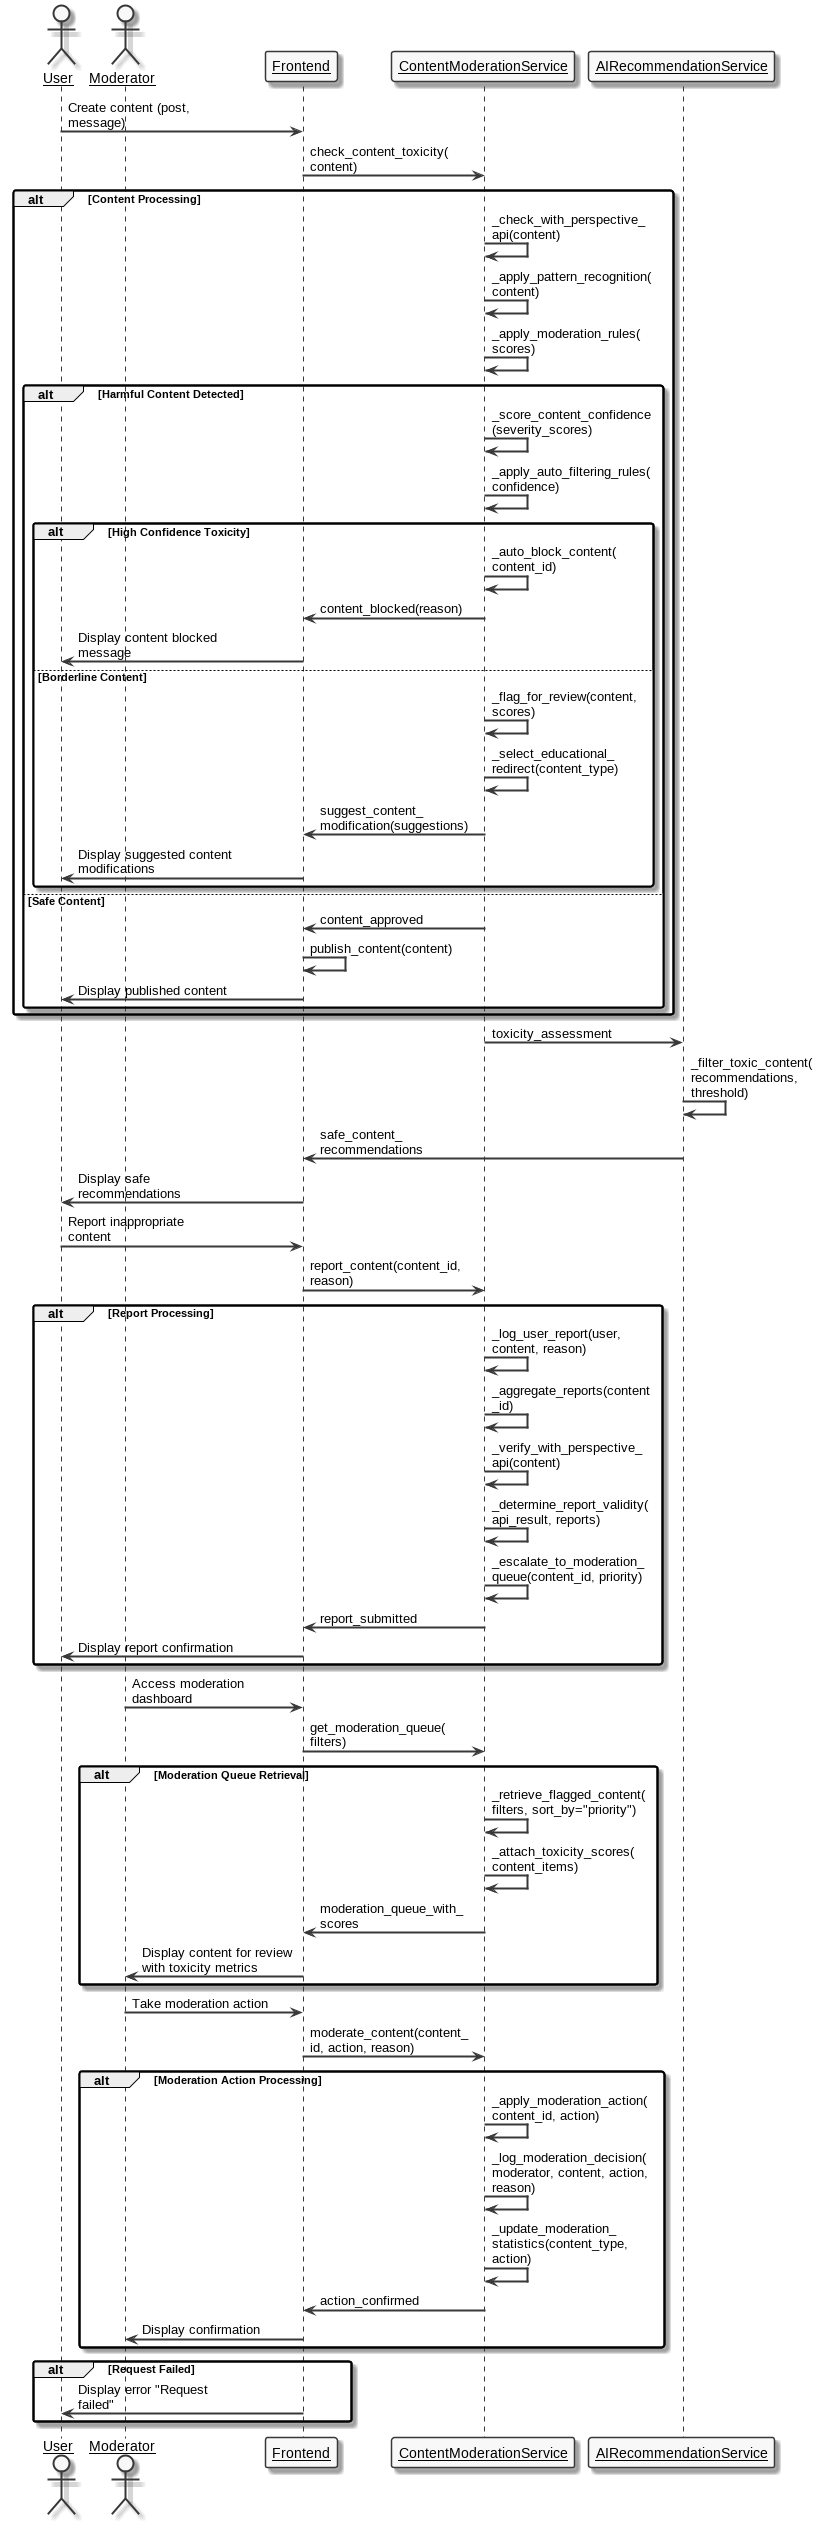
\includegraphics[width=0.52\textwidth]{images/chapter 5/sprint 4/Moderation_Sequence_Diagram.png}
    \caption{Toxic Content Detection - Content Moderation}
    \label{fig:moderation-sequence-diagram}
\end{figure}

\begin{figure}[H]
    \centering
    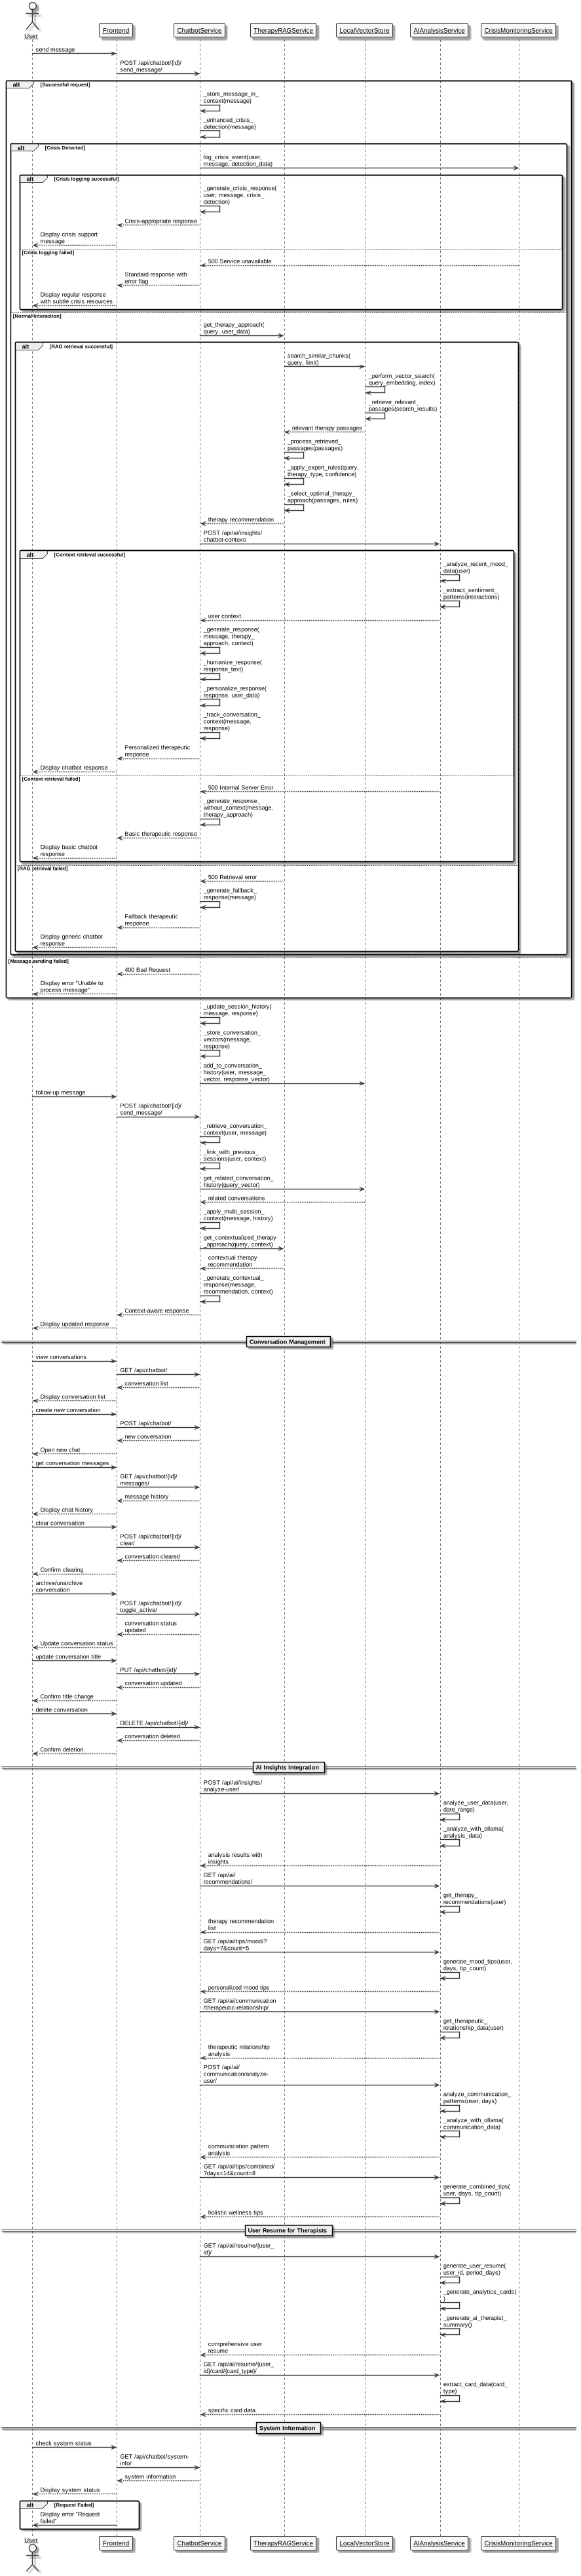
\includegraphics[width=0.42\textwidth]{images/chapter 5/sprint 4/Chatbot_Sequence_Diagram.png}
    \caption{Enhanced Chatbot with RAG System}
    \label{fig:chatbot-sequence-diagram}
\end{figure}

\begin{figure}[H]
    \centering
    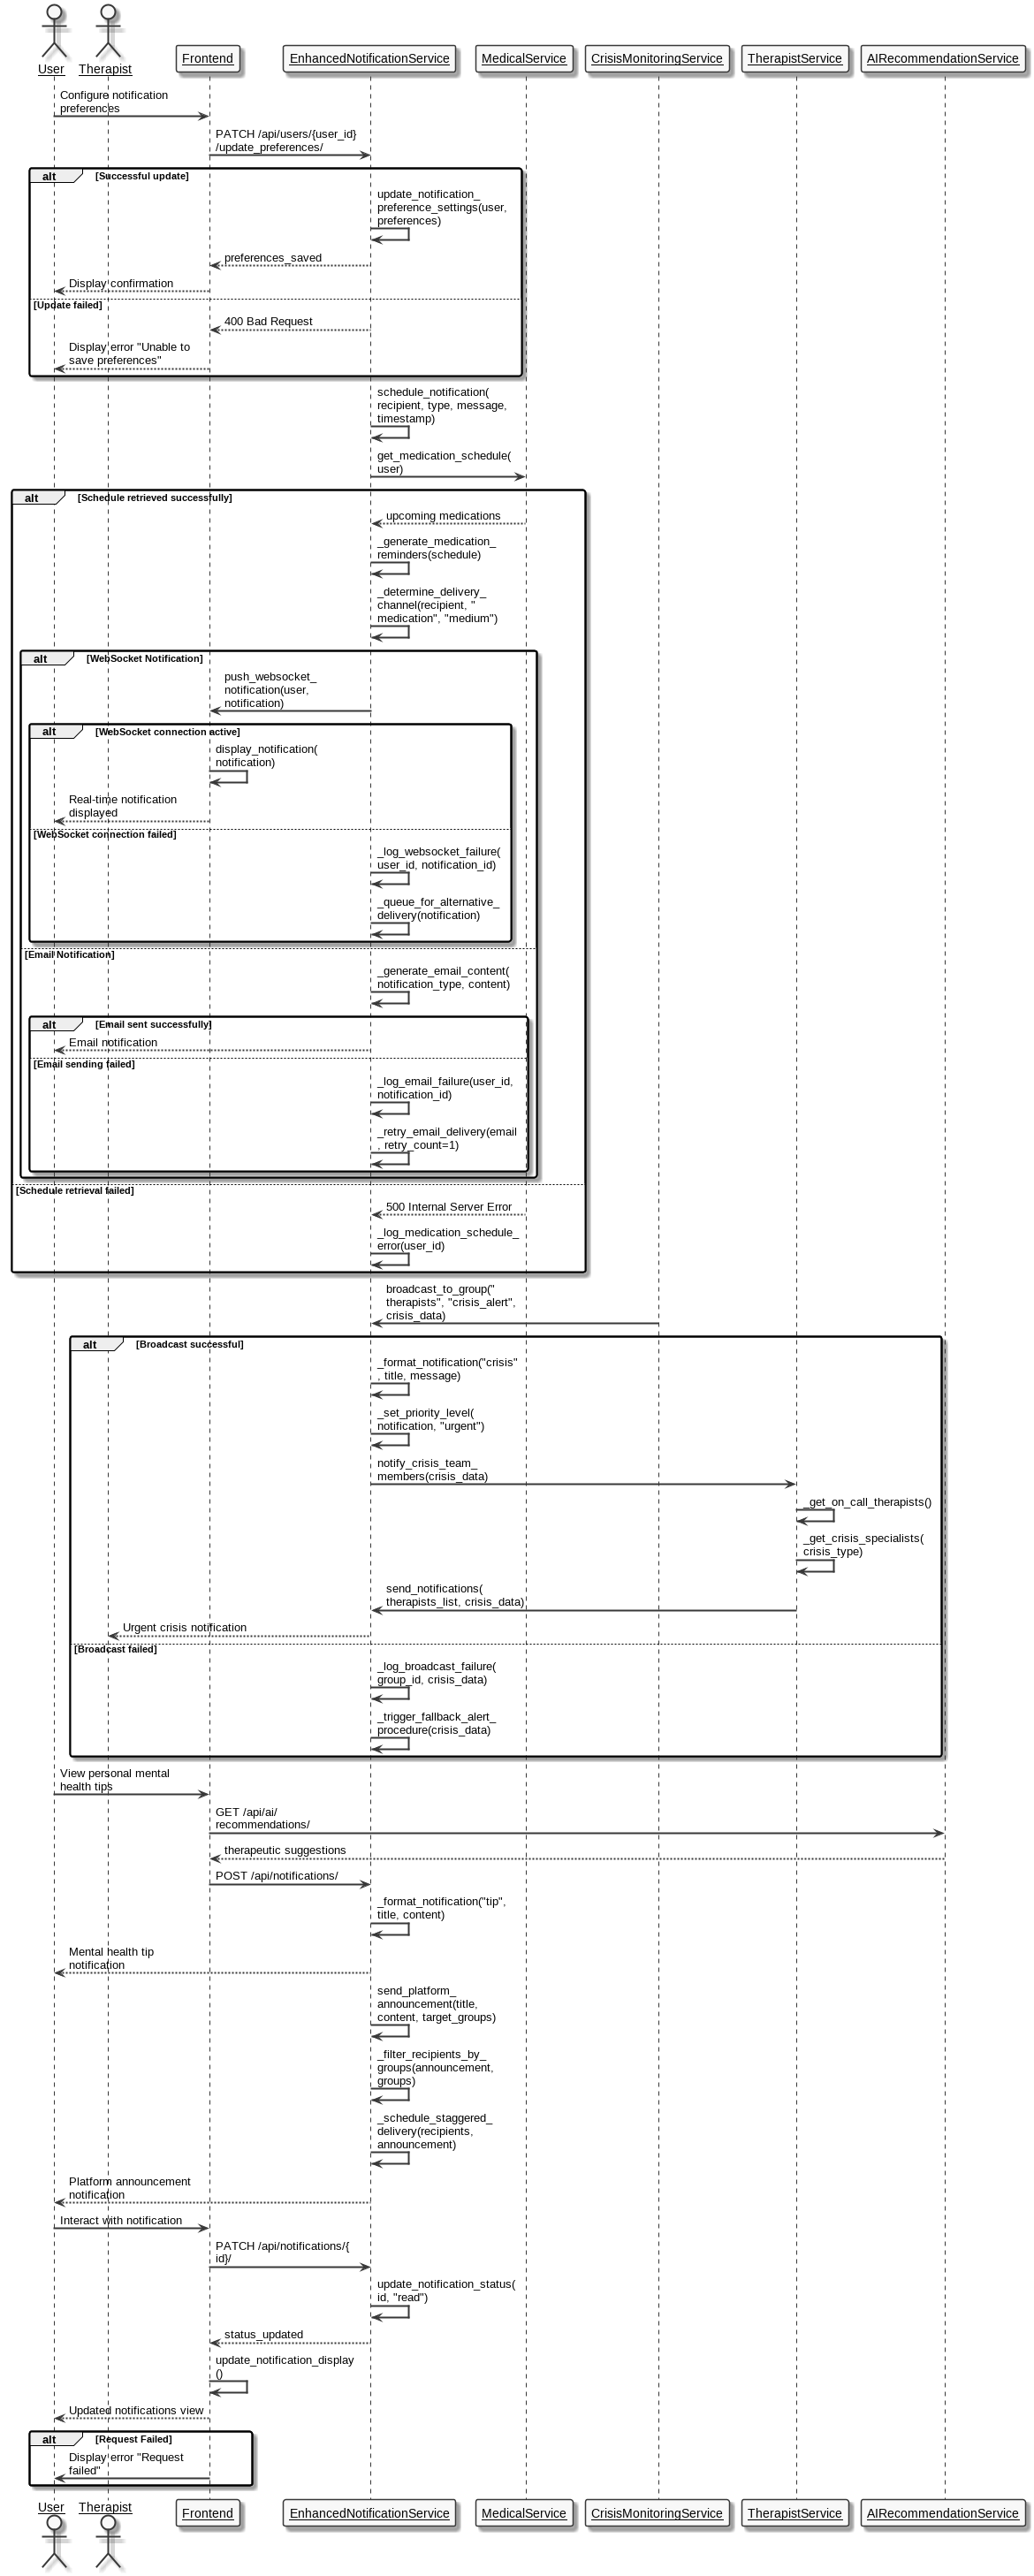
\includegraphics[width=0.75\textwidth]{images/chapter 5/sprint 4/Notifications_Sequence_Diagram.png}
    \caption{Enhanced Notifications System}
    \label{fig:notifications-sequence-diagram}
\end{figure}
